\documentclass{beamer}
%
% Choose how your presentation looks.
%
% For more themes, color themes and font themes, see:
% http://deic.uab.es/~iblanes/beamer_gallery/index_by_theme.html
%
\mode<presentation>
{
  \usetheme{Darmstadt}      % or try Darmstadt, Madrid, Warsaw, ...
  \usecolortheme{default} % or try albatross, beaver, crane, ...
  \usefonttheme{default}  % or try serif, structurebold, ...
%   \setbeamertemplate{navigation symbols}{}
  \setbeamertemplate{caption}[numbered]
}

%New colors defined below
\definecolor{codegreen}{rgb}{0,0.6,0}
\definecolor{codegray}{rgb}{0.5,0.5,0.5}
\definecolor{codepurple}{rgb}{0.58,0,0.82}
\definecolor{backcolour}{rgb}{0.95,0.95,0.92}
\definecolor{Gray}{gray}{0.9}


\usepackage[english]{babel}
\usepackage[utf8x]{inputenc}
\usepackage{amsmath}
\usepackage{subfigure}
\usepackage{caption}
\usepackage{amsthm}
\usepackage{amsmath}
\usepackage{algorithm}
\usepackage{algpseudocode}
\usepackage{pifont}
\usepackage{listings}
\usepackage{xcolor}
\usepackage{tikz}
\usepackage{colortbl}
\usepackage[export]{adjustbox}

\usetikzlibrary{matrix}
\newcommand{\tikzmark}[2]{\tikz[overlay, remember picture] \node[inner sep=0pt, outer sep=0pt, anchor=base] (#1) {#2};}
\newcolumntype{g}{>{\columncolor{Gray}}c}


%Code listing style named "mystyle"
\lstdefinestyle{mystyle}{
  backgroundcolor=\color{backcolour},
  commentstyle=\color{codegreen},
  keywordstyle=\color{magenta},
  numberstyle=\tiny\color{codegray},
  stringstyle=\color{codepurple},
  basicstyle=\ttfamily\footnotesize,
  breakatwhitespace=false,         
  breaklines=true,                 
  captionpos=b,                    
  keepspaces=true,                 
  numbers=left,                    
  numbersep=5pt,                  
  showspaces=false,                
  showstringspaces=false,
  showtabs=false,                  
  tabsize=2
}

\DeclareMathOperator*{\argmax}{arg\,max}
\newtheorem*{remark}{Remark}

\title[]{AI and ML: Introduction and Beyond}
\author{Varad Meru}
\institute{Azure Functions, App Services,\newline Microsoft Corp.\newline\newline}
\date{}

% \newline \raisebox{-0.40ex}{
\includegraphics[width=2.5ex]{LinkedIn-InBug-2C.png}} \href{https://www.linkedin.com/in/vmeru}{\texttt{ linkedin.com/in/vmeru}}\newline\raisebox{-0.40ex}{
\includegraphics[width=2.5ex]{Octocat.png}}\href{https://github.com/vrdmr}{\texttt{ github.com/vrdmr}}\newline\raisebox{-0.40ex}{
\includegraphics[width=2.5ex]{Twitter_logo_blue.png}}\href{https://twitter.com/vrdmr}{\texttt{ @vrdmr}}}

%"mystyle" code listing set
\lstset{style=mystyle}

\begin{document}
\begin{frame}
   \titlepage
   \begin{table}[]
\begin{tabular}{l l}
{
\includegraphics[width=2.5ex]{LinkedIn-InBug-2C.png}}  \href{https://www.linkedin.com/in/vmeru}{\texttt{ linkedin.com/in/vmeru}}\\
\raisebox{-0.40ex}{
\includegraphics[width=2.5ex]{Octocat.png}}  \href{https://github.com/vrdmr}{\texttt{ github.com/vrdmr}} \\
\raisebox{-0.40ex}{
\includegraphics[width=2.5ex]{Twitter_logo_blue.png}}  \href{https://twitter.com/vrdmr}{\texttt{ @vrdmr}} \\
\end{tabular}
\end{table}
\end{frame}

\section{Background}
\label{sec:Background}
\begin{frame}{Who am I}
\begin{itemize}
    \item Current: Senior SDE @ Microsoft Corp.
    \begin{itemize}
    \item Working on Python Azure Functions.
    \item Previously worked on Compute Platform within Azure Core.
    \end{itemize}
    \item Previous Experiences:
    \begin{itemize}
    \item Worked for Orzota (Chennai) and Persistent Systems (Pune).
    \item Internship experiences at Facebook and Nomura.
    \end{itemize}
    \item Education:
    \begin{itemize}
    \item MS in CS (ML and Data Systems) from UC Irvine (2015)
    \item BE in CSE from Shivaji University (DYPCET) (Class of 2011)
    \end{itemize}
    \item Interests: Distributed Systems \& Cloud Infra, ML, Economics.
\end{itemize}
\begin{figure}
\centering
\captionsetup{justification=centering}

\includegraphics[scale=0.35]{Picture1.png}
\end{figure}
\end{frame}

%%%%%%%%%%%%%%%%%%%%%%
%%%% Outline Section
%%%%%%%%%%%%%%%%%%%%%%
\section{Outline}
\begin{frame}{Outline}
\begin{itemize}
  \item \nameref{sec:Introduction}
  \item \nameref{sec:HistoryOfAI} and \nameref{sec:AILandscape}
  \item \nameref{sec:MLintroduction}
  \item \nameref{sec:GettingStartedInML}
\end{itemize}
\end{frame}

%%%%%%%%%%%%%%%%%%%%%%
% Introduction Section
%%%%%%%%%%%%%%%%%%%%%%

\section{Introduction}
\label{sec:Introduction}
\begin{frame}{Introduction}

{\large Q. What is artificial intelligence?}
\newline\newline
{\large A. It is the science and engineering of making intelligent machines, especially intelligent computer programs. \newline\newline It is related to the similar task of using computers to understand human intelligence, but AI does not have to confine itself to methods that are biologically observable.}
\end{frame}

\begin{frame}[allowframebreaks]{AI Examples}
{\large Here are some examples which give us the perception of AI}
\begin{figure}
\centering
\captionsetup{justification=centering}
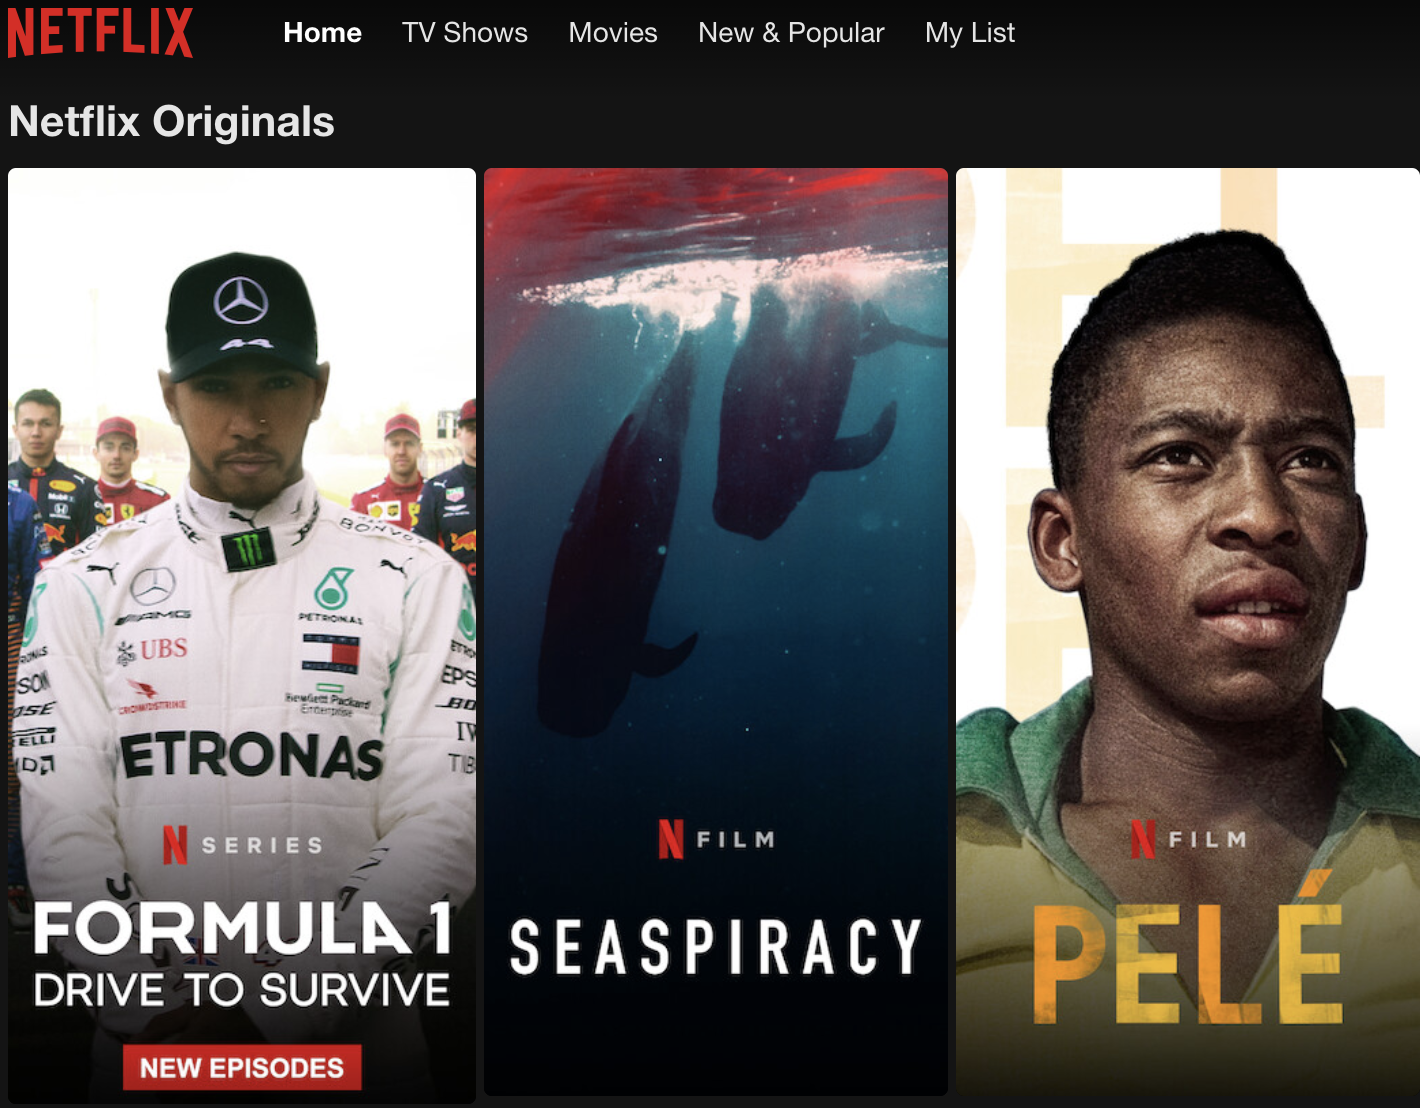
\includegraphics[scale=0.30]{NFLX.png}
\caption{Netflix Recommendations}
\end{figure}
\framebreak
\begin{figure}
\centering
\captionsetup{justification=centering}
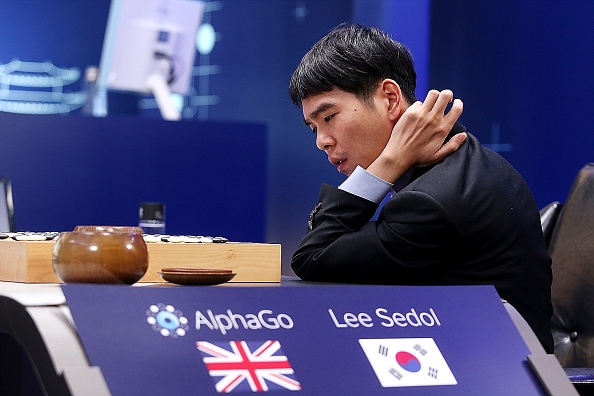
\includegraphics[scale=0.30]{alphago.jpeg}
\caption{AlphaGo vs Lee Sedol}
\end{figure}
\framebreak
\begin{figure}
\centering
\captionsetup{justification=centering}
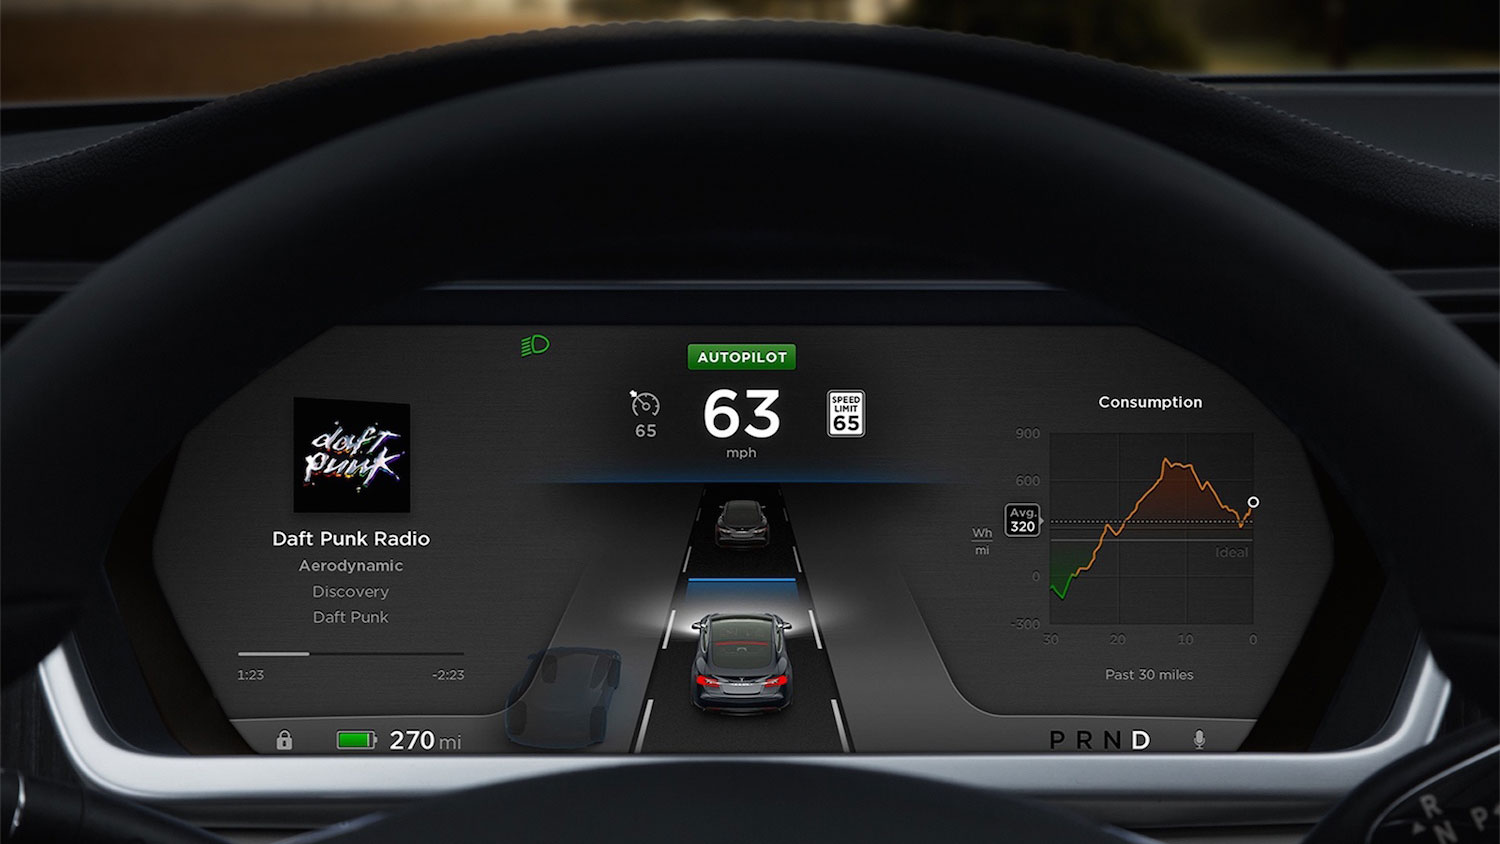
\includegraphics[scale=0.20]{autopilot.jpeg}
\caption{Tesla Autopilot}
\end{figure}
\framebreak
\begin{figure}
\centering
\captionsetup{justification=centering}
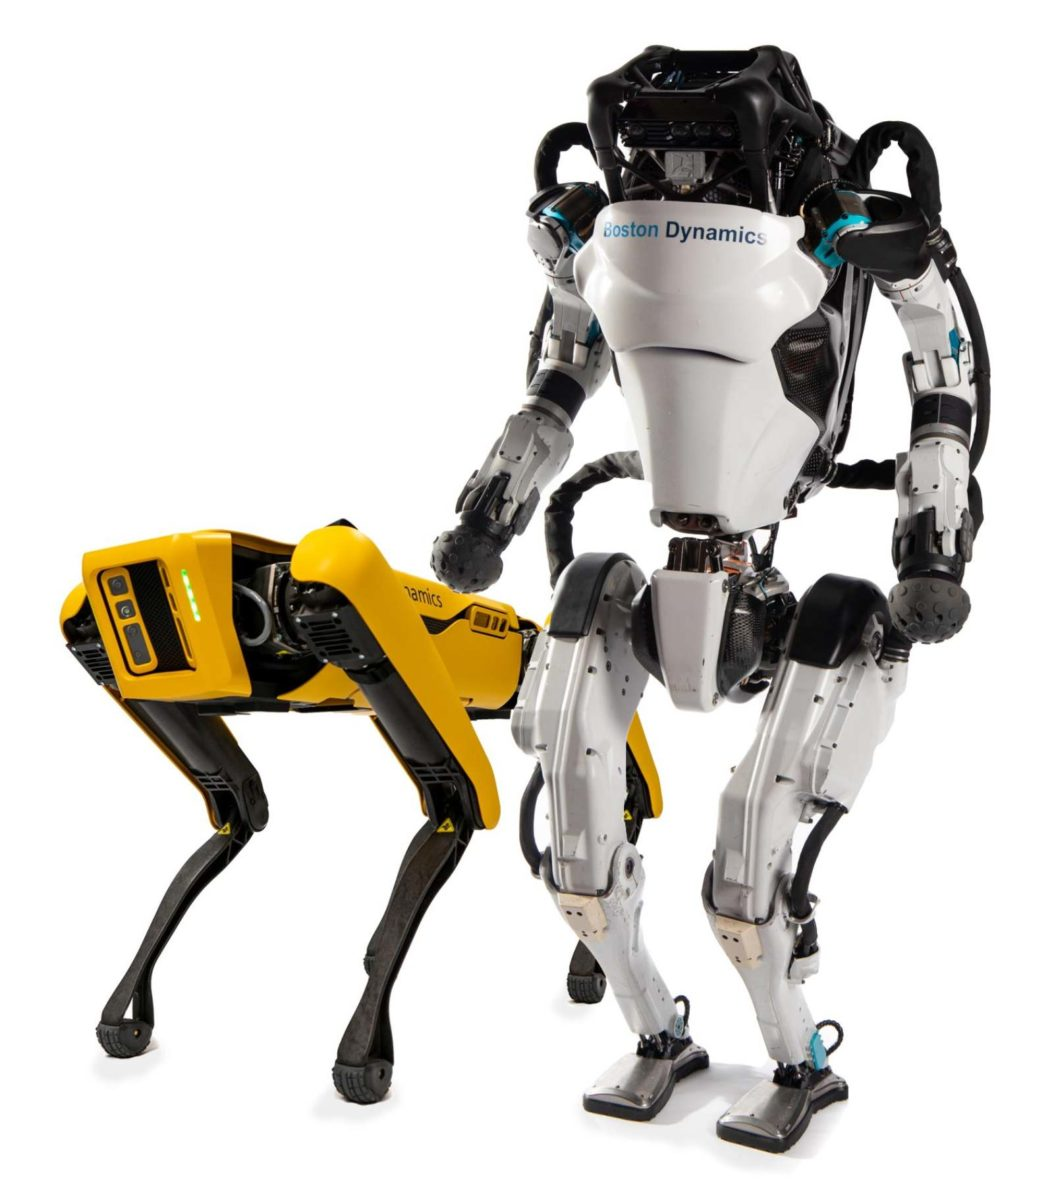
\includegraphics[scale=0.60]{BDExample.jpeg}
\caption{Robot from Boston Dynamics}
\end{figure}
\end{frame}

\section{History of AI}
\label{sec:HistoryOfAI}
\begin{frame}[allowframebreaks]{History of AI}

\begin{itemize}
\item 1940’s — Interest in neurons, neural networks and their relationship to mathematics and learning
\item 1950 — Turing’s paper
\item 1956 — Dartmouth conference (Defining AI)
\item 1950’s and 1960’s — enthusiasm and optimism; big promises
\item Late 1960’s and 1970’s — Realization that further progress was really hard; disillusionment
\item 1980’s — Expert Systems, neural networks, etc.; AI now a little different; quiet successes
\item 1990’s — Intelligent agents, probabilistic reasoning, machine learning, DeepBlue.
\item 2000’s — robot pets, self-driving cars.
\item 2010’s — Deep Learning, AlexNet, AlphaGo, GPT-3.
\end{itemize}
\end{frame}

\begin{frame}{Calls for clarity}
\begin{figure}
\centering
\captionsetup{justification=centering}
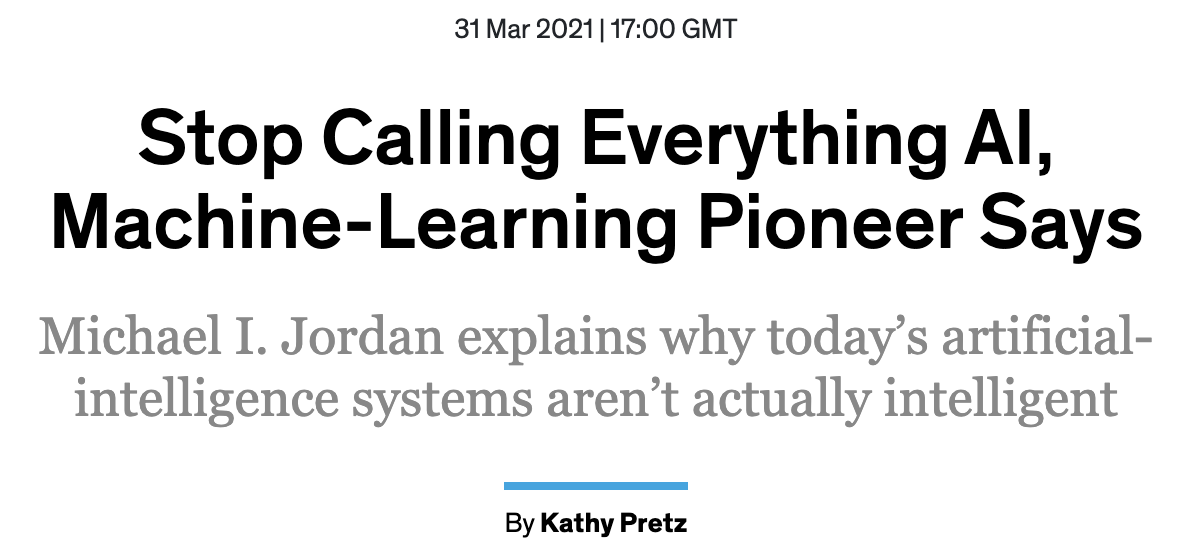
\includegraphics[scale=0.30]{AInotML1.png}
\end{figure}
\begin{figure}
\centering
\captionsetup{justification=centering}
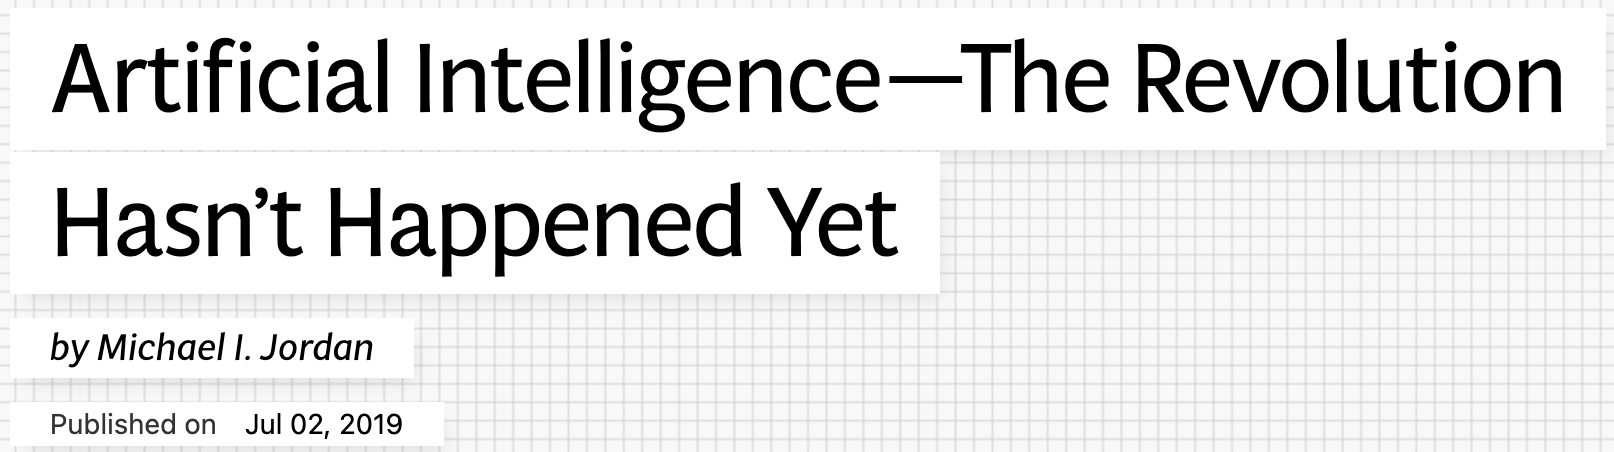
\includegraphics[scale=0.30]{AInotML2.png}
\end{figure}
\end{frame}

\section{Landscape}
\label{sec:AILandscape}
\begin{frame}[allowframebreaks]{AI Landscape}
\begin{itemize}
\item Knowledge representation (including formal logic)
\item Search, especially heuristic search (puzzles, games)
\item Planning
\item Reasoning under uncertainty, including probabilistic reasoning
\item Learning
\item Agent architectures
\item Robotics and perception
\item Natural language processing
\end{itemize}
\framebreak
{\large Example: Search}\\
Solving search Problems using \texttt{minmax} adversarial search
\begin{figure}
\centering
\captionsetup{justification=centering}
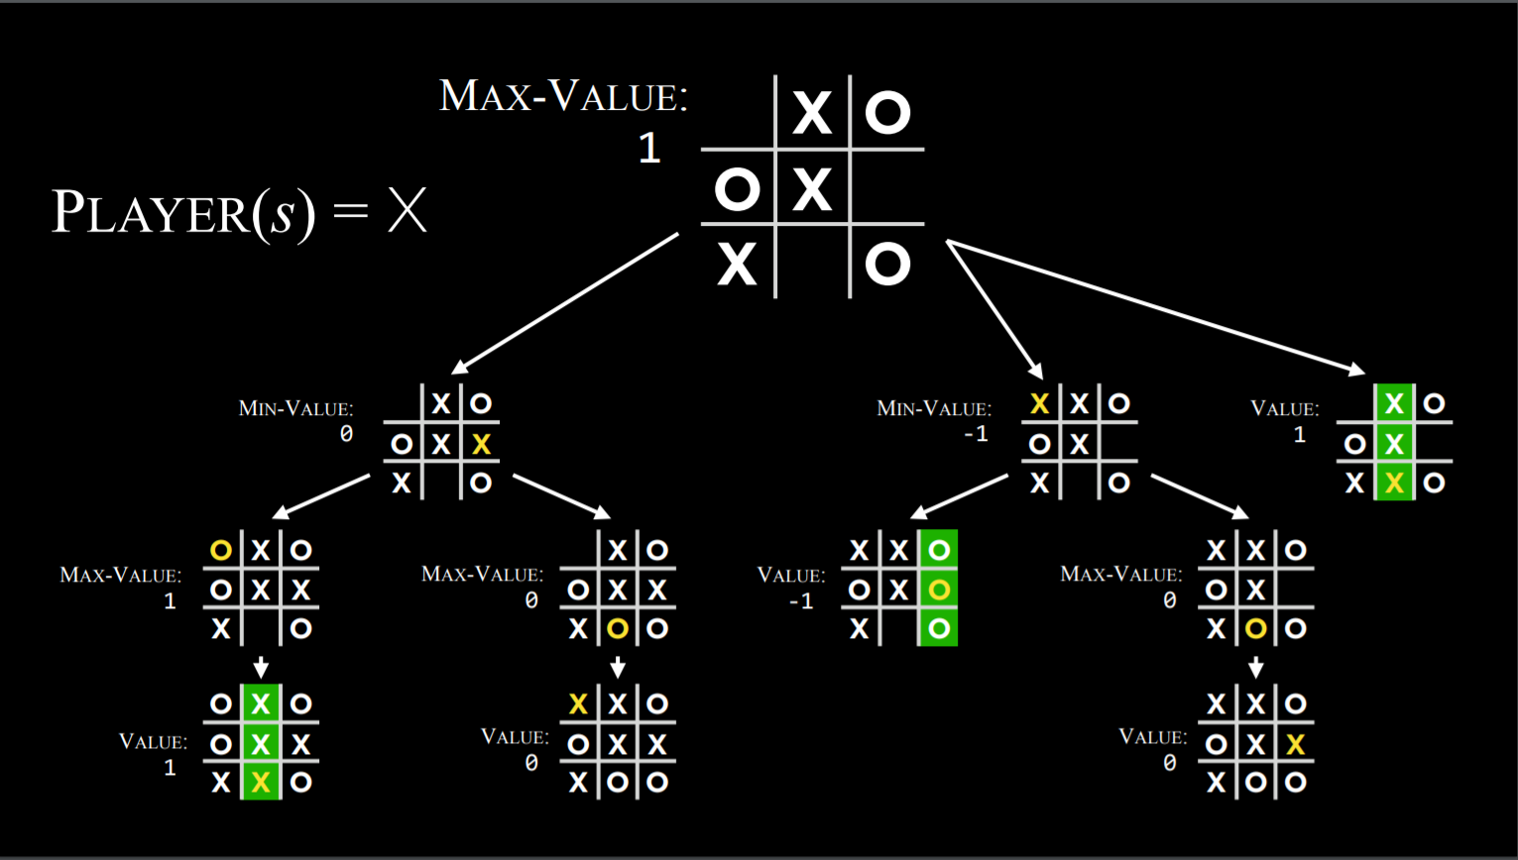
\includegraphics[scale=0.30]{minimax_tictactoe.png}
\end{figure}
\framebreak
{\large Example: Predicting under Uncertainty - Markov Chains}\\
To start constructing a Markov chain, we need a \textbf{transition model}
\begin{figure}
\centering
\captionsetup{justification=centering}
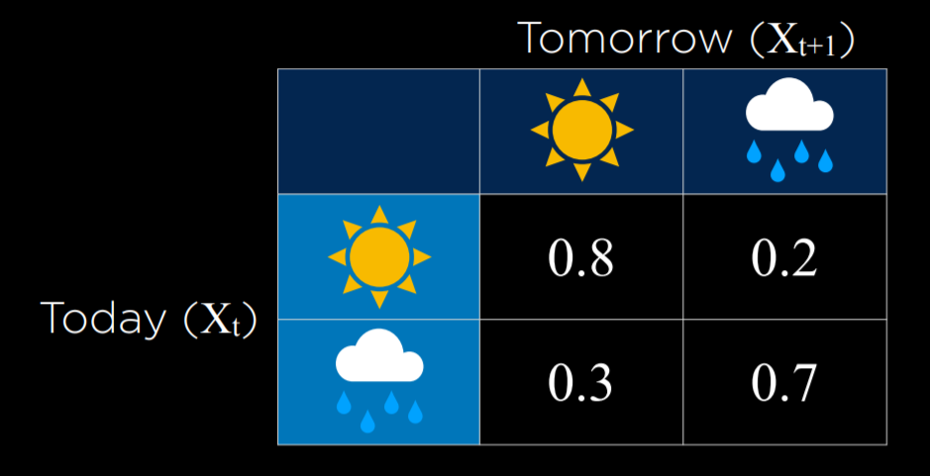
\includegraphics[scale=0.25]{transitionmodel.png}
\end{figure}
We can now answer questions such as \textit{“what is the probability of having four rainy days in a row?”}
\begin{figure}
\centering
\captionsetup{justification=centering}
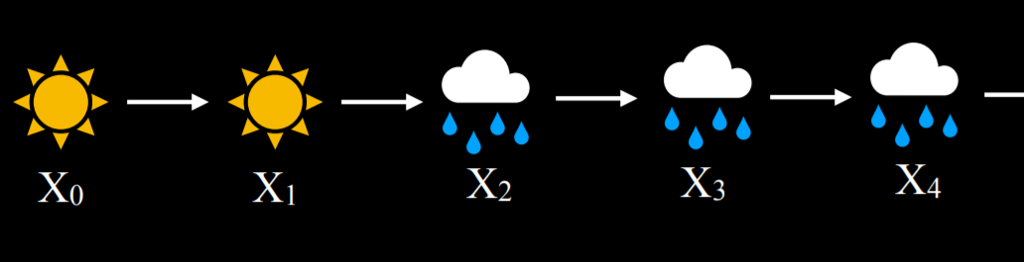
\includegraphics[scale=0.30]{markovchain.png}
\end{figure}
\framebreak
\begin{itemize}
\item Knowledge representation (including formal logic)
\item Search, especially heuristic search (puzzles, games)
\item Planning
\item Reasoning under uncertainty, including probabilistic reasoning
\item \textbf{Learning}: \textit{The main driver of recent successes in AI}
\item Agent architectures
\item Robotics and perception
\item Natural language processing
\end{itemize}
\end{frame}

\section{Introduction to Machine Learning}
\label{sec:MLintroduction}
\begin{frame}[allowframebreaks]{What is ML?}
Machine learning algorithms are data analysis methods which search data sets for patterns and characteristic structures.
\framebreak
\newline\newline
Paradigms:
\begin{itemize}
    \item \textit{Modeling}: Modeling is the process of approximating real world problems using formal mathematical objects called \textbf{models},
    \item \textit{Inference}: Given a model, the task of \textbf{inference} is to answer questions about model.
    \item \textit{Learning}: Machine learning is this process of turning an abstract model family that we can easily write down into a concrete model of the world that we can query
\end{itemize}
\framebreak
\begin{figure}
\centering
\captionsetup{justification=centering}
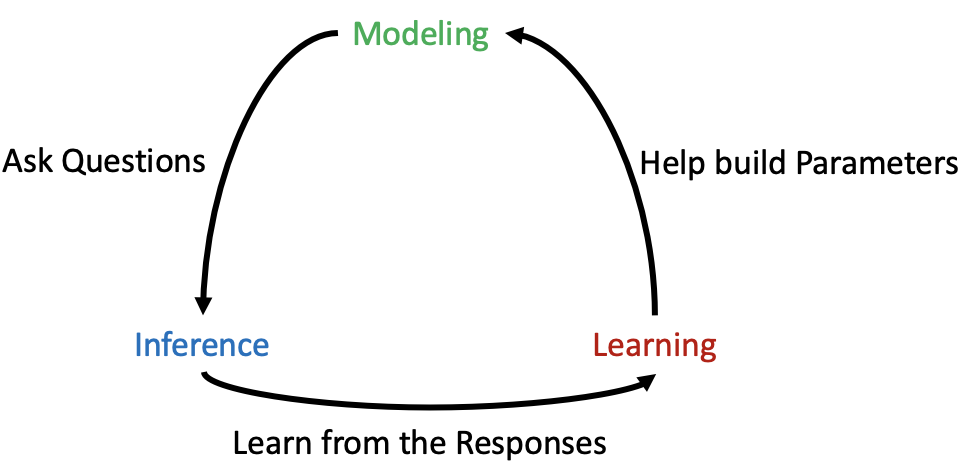
\includegraphics[scale=0.50]{Paradigm.png}
\end{figure}
\end{frame}

\begin{frame}[allowframebreaks]{ML Algorithms}
Types of Prediction problems:
\begin{itemize}
\item Supervised Learning
\begin{itemize}
    \item “Labeled” training data
    \item Every example has a desired target value (a “best answer”)
    \item Reward prediction being close to target
    \item[] Examples
    \begin{itemize}
    \item Classification: a discrete-valued prediction (often: action / decision)
    \item Regression: a continuous-valued prediction
    \end{itemize}
\end{itemize}
\end{itemize}

\begin{figure}
\centering
\captionsetup{justification=centering}
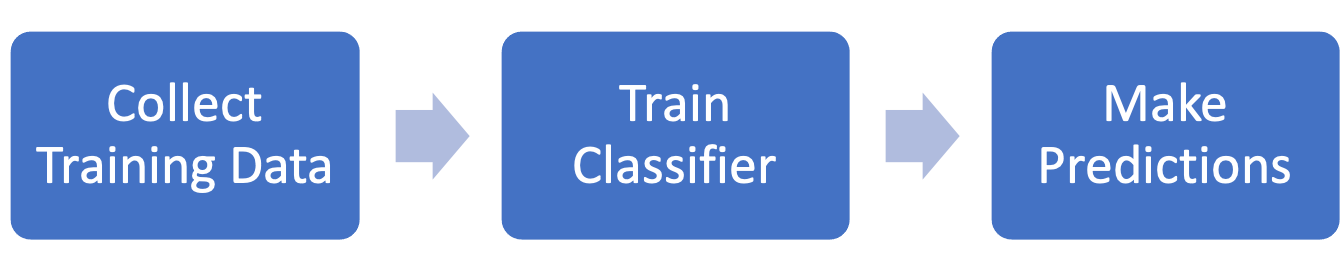
\includegraphics[scale=0.45]{SupervisedLearning.png}
\end{figure}

\framebreak
\subsection{Supervised Learning}
\begin{itemize}
\item Supervised Learning: Some Algorithms
\begin{itemize}
    \item Classification: a discrete-valued prediction
    \begin{itemize}
        \item K-Nearest Neighbors (KNN)
        \item Support Vector Machines (SVM)
        \item Decision Trees
        \item Naïve Bayes Classifiers
        \item Logistic Regression
    \end{itemize}
    \item Regression: a continuous-valued prediction
    \begin{itemize}
        \item Linear Regression
        \item Poisson Regression
    \end{itemize}
\end{itemize}
\item Supervised Learning: Applications
    \begin{itemize}
        \item Spam Detection
        \item Speech Recognition
        \item Handwriting Recognition
        \item Information Retrieval
    \end{itemize}
\end{itemize}

\framebreak
{\large Example - Decision Tree Classifier}
\begin{table}[]
\begin{tabular}{||g c | c||}
 \hline
 Weight & Texture & Label \\ [0.5ex] 
 \hline\hline
 150g & Bumpy & Orange \\ \hline
 170g & Bumpy & Orange \\ \hline\rowcolor{Gray}
 130g & Smooth & Apple \\ \hline
 140g & Smooth & Apple \\ \hline
 ... & ... & ... \\
\hline
\end{tabular}
\caption{Fruit Classification Dataset}
\end{table}

\framebreak
{\large Example - Decision Tree Classifier}
\begin{figure}
\centering
\captionsetup{justification=centering}
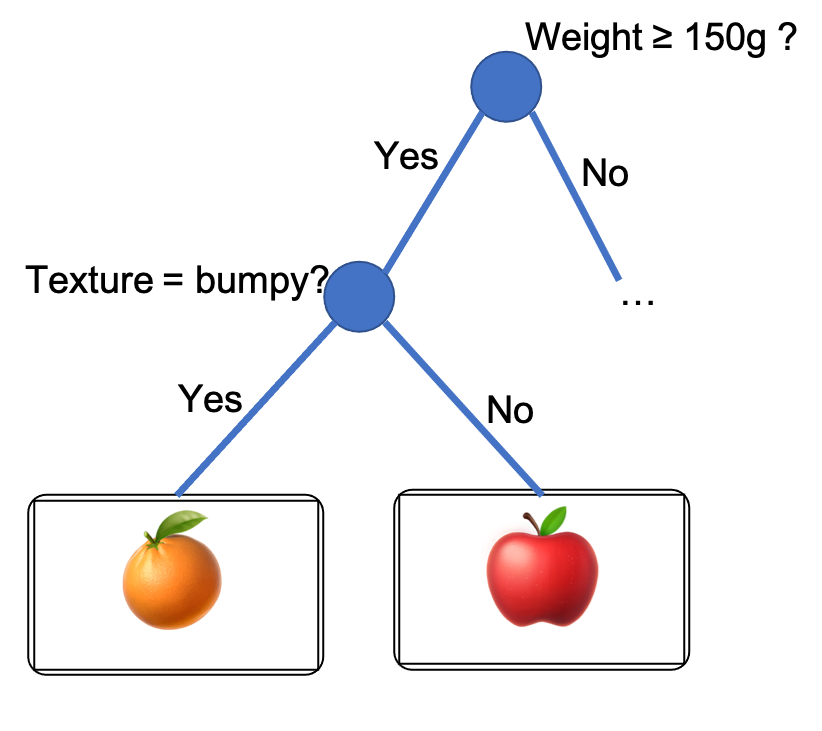
\includegraphics[scale=0.45]{DecisionTree.png}
\end{figure}

\framebreak
{\large Example - Decision Tree Classifier}
\begin{lstlisting}
HelloWorldForScikitLearn

from sklearn import tree

label\_map = \{1: "Apple", 0: "Orange"\}

features = [[140, 1], 
            [130, 1], 
            [150, 0], 
            [170, 0]]

labels = [0,
          0,
          1,
          1]

clf = tree.DecisionTreeClassifier()

clf = clf.fit(features, labels)

prediction = clf.predict([[150, 0]])[0]

print(label\_map[prediction])
\end{lstlisting}

\framebreak
\subsection{Unsupervised Learning}
Types of Prediction problems:
\begin{itemize}
\item Supervised Learning
\item Unsupervised Learning
\begin{itemize}
    \item Data has lots of rich latent structures; want methods to discover this structure automatically.
    \item No known target value
    \item No targets = nothing to predict?
    \item Reward “patterns” or “explaining features”
    \item Often, data mining
\end{itemize}
\end{itemize}

\framebreak
\begin{itemize}
\item Unsupervised Learning: Some Algorithms
\begin{itemize}
    \item Clustering
    \begin{itemize}
        \item Hierarchical clustering
        \item k-means
    \end{itemize}
    \item Anomaly Detection
    \begin{itemize}
        \item Local Outlier Factor
        \item Isolation Forest
    \end{itemize}
    \item Learning latent variable models
    \begin{itemize}
        \item Expectation–maximization algorithms (EM)
        \item PCA and SVD
    \end{itemize}
    \item Neural Nets: Hopfield, Boltzmann and RBMs, and Auto-Encoders
\end{itemize}
\item Unsupervised Learning: Applications
    \begin{itemize}
        \item Pattern Recognition
        \item Grouping
        \item Feature Engineering
    \end{itemize}
\end{itemize}

\framebreak
{\large Example - KMeans Clustering}
\begin{figure}
\centering
\captionsetup{justification=centering}
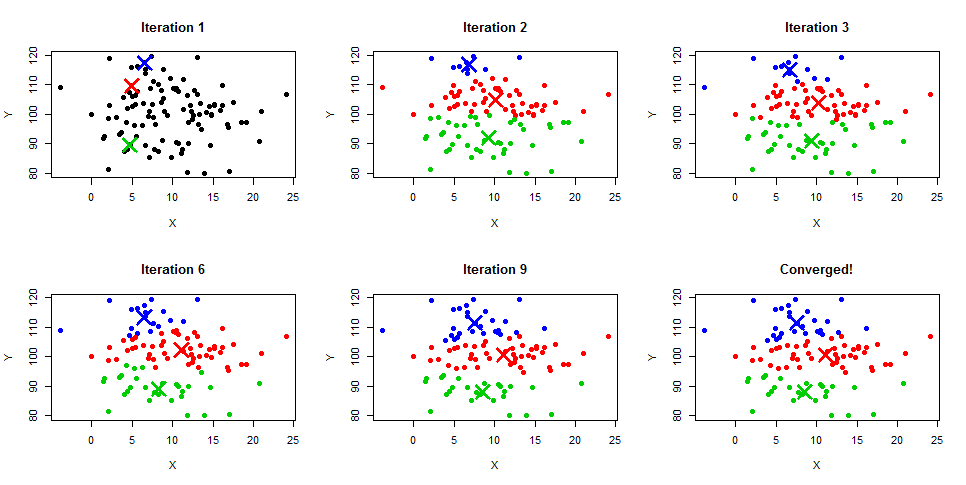
\includegraphics[scale=0.33]{kmeans-example.png}
\end{figure}

\framebreak
\begin{figure}
\centering
\captionsetup{justification=centering}
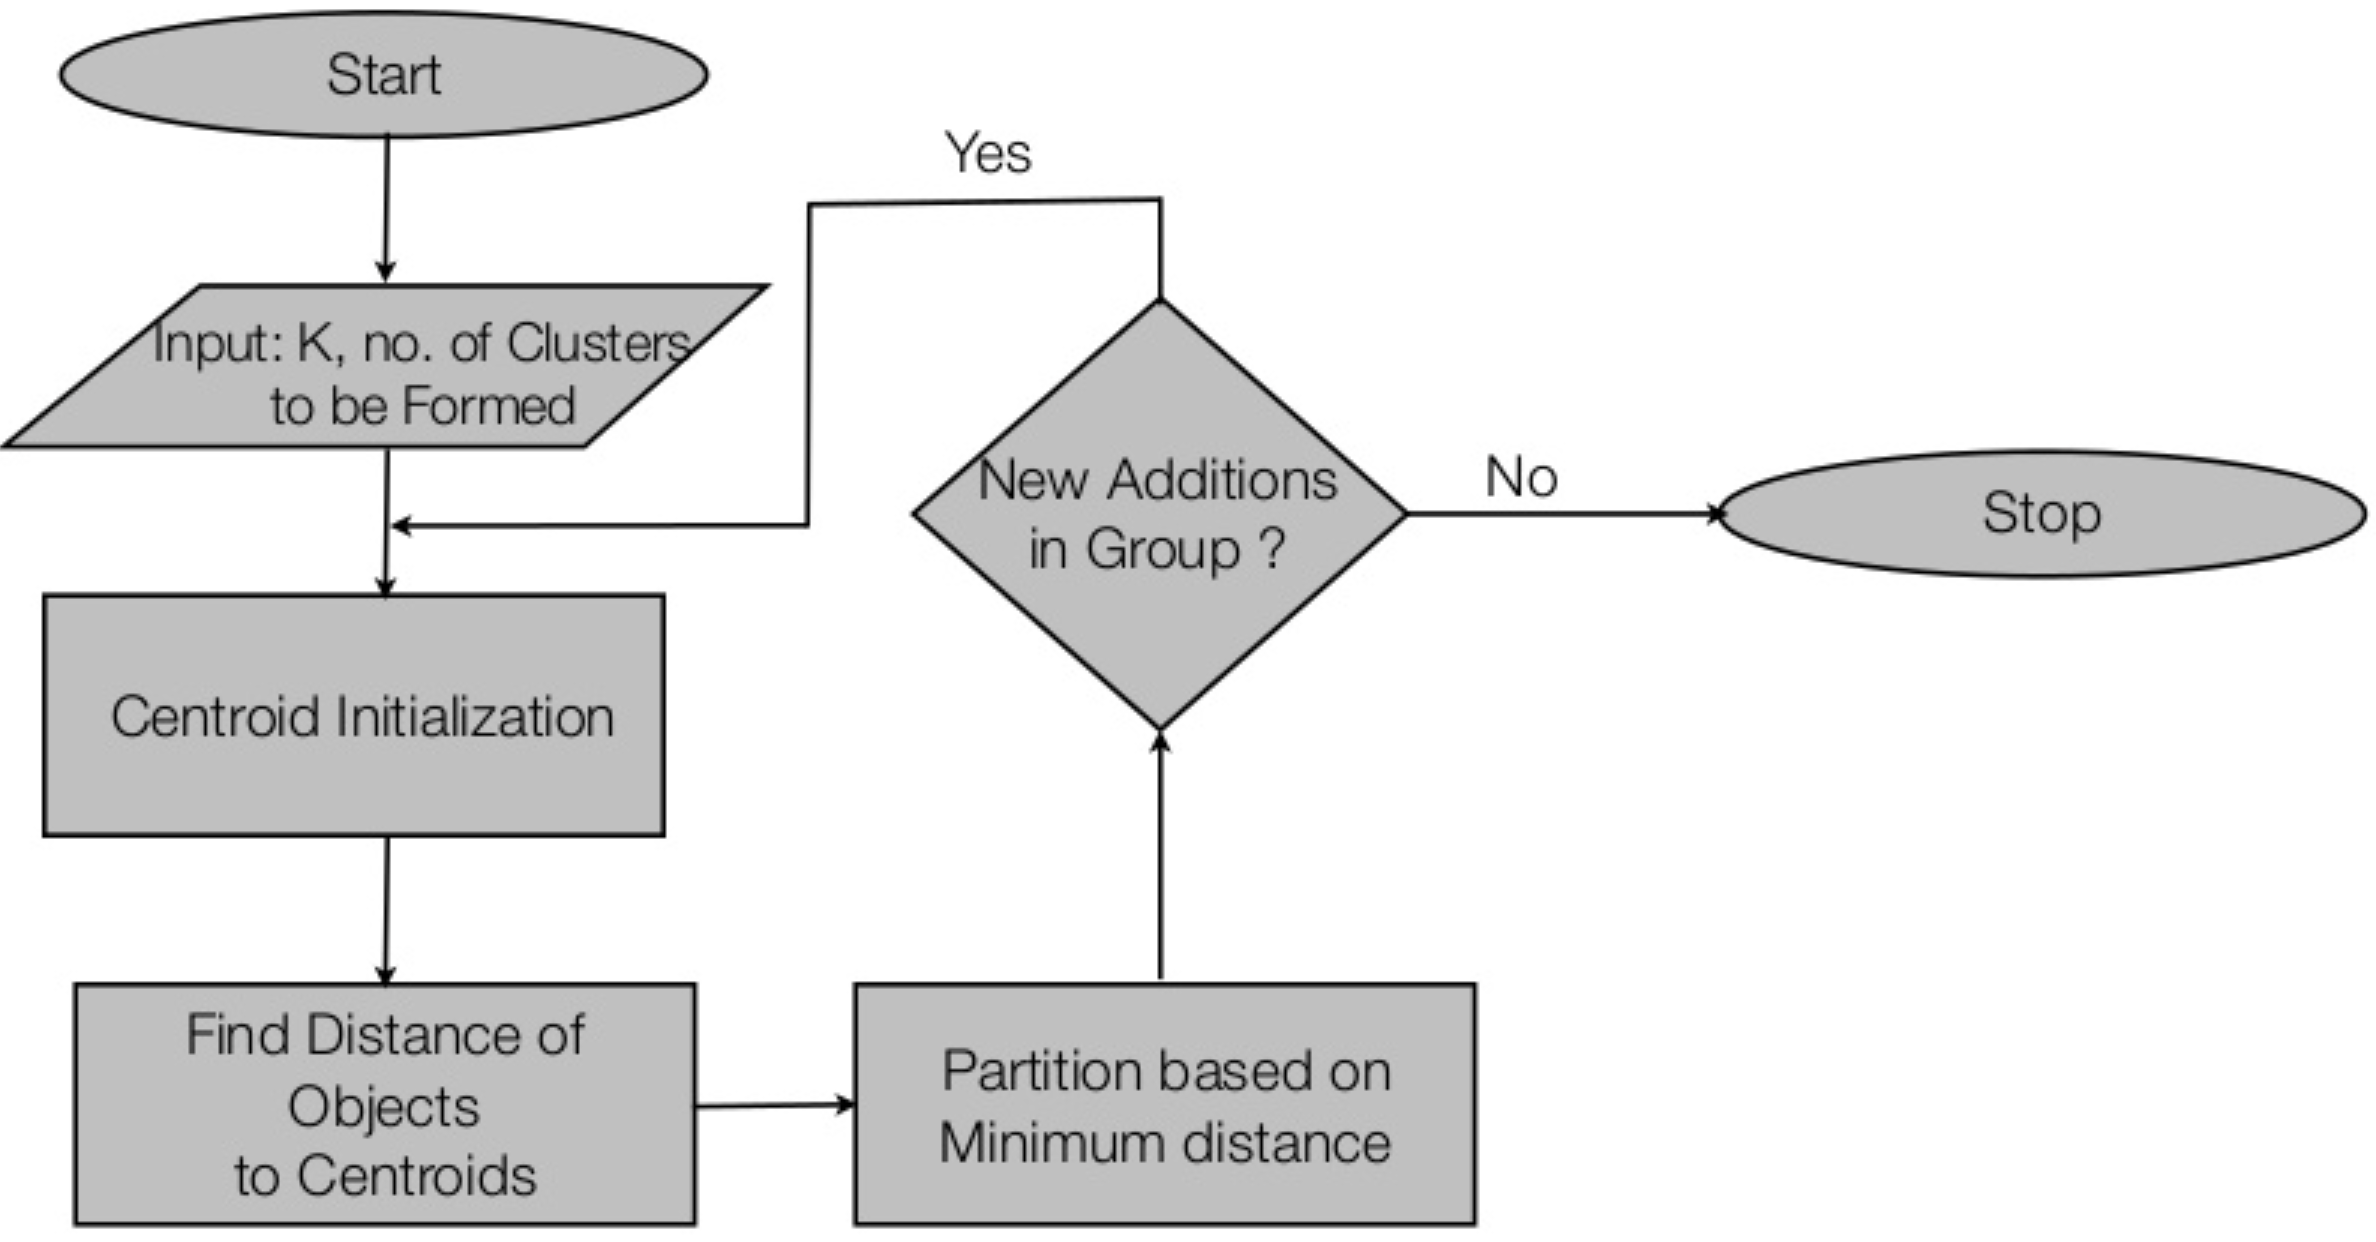
\includegraphics[scale=0.23]{KMeans.png}
\end{figure}

\framebreak

{\large Example - KMeans Clustering}
\begin{lstlisting}
kmeans-example

from sklearn.datasets import make\_blobs

from sklearn.cluster import KMeans

\# create dataset

X, y = make\_blobs(n\_samples=150, n\_features=2,
        centers=3, cluster\_std=0.5,
        shuffle=True,random\_state=0)

km = KMeans(n\_clusters=3, init='random',
            n\_init=10, max\_iter=300,
            tol=1e-04, random\_state=0)

y\_km = km.fit\_predict(X)
\end{lstlisting}

\framebreak
\subsection{Semi-supervised Learning}
Types of Prediction problems:
\begin{itemize}
\item Supervised Learning
\item Unsupervised Learning
\item Semi-supervised learning
\begin{itemize}
    \item Similar to supervised
    \item Some data have unknown target values
    \item[] Examples
    \begin{itemize}
    \item Medical data - Lots of patient data, few known outcomes
    \item Image tagging - Lots of images on Flikr/Facebook, but only some of them tagged
    \end{itemize}
\end{itemize}
\end{itemize}

\framebreak
\subsection{Reinforcement Learning}
Types of Prediction problems:
\begin{itemize}
\item Supervised Learning
\item Unsupervised Learning
\item Semi-supervised learning
\item Reinforcement learning
\begin{itemize}
    \item “Indirect” feedback on quality - No answers, just “better” or “worse”
    \item Feedback may be delayed
\end{itemize}
\end{itemize}
\begin{figure}
\centering
\captionsetup{justification=centering}
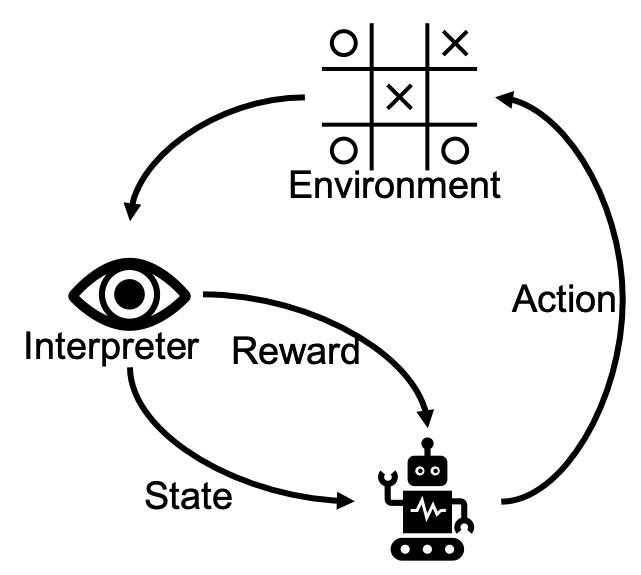
\includegraphics[scale=0.3]{RLDiag.png}
\end{figure}
\end{frame}

\subsection{Tools and Libraries}
\begin{frame}{Tools and Libraries (Python)}
\begin{itemize}
    \item \href{https://scikit-learn.org/stable/index.html}{Scikit-learn: best library for classical ML algorithms: \texttt{scikit-learn.org}}
    \item \href{https://www.tensorflow.org/}{Tensorflow: Machine Learning and Deep Learning library: \texttt{tensorflow.org}}
    \item \href{https://pandas.pydata.org/}{Pandas: data extraction and preparation: \texttt{pandas.pydata.org}}
    \item \href{https://numpy.org/}{NumPy: arrays and linear algebra library: \texttt{numpy.org}}
    \item \href{https://www.scipy.org/}{SciPy: scientific computing library: \texttt{scipy.org}}
    \item \href{https://matplotlib.org/}{Matplotlib: plotting and data visualization: \texttt{matplotlib.org}}
    \item \href{https://pytorch.org/}{PyTorch: alternative Deep Learning library: \texttt{pytorch.org}}
    \item \href{https://keras.io/}{Keras: high-level wrapper around TensorFlow: \texttt{keras.io}}
\end{itemize}
\end{frame}

\section{ML Pyramid}
\label{sec:MLPyramid}
\begin{frame}{ML Pyramid}
\begin{figure}
\centering
\captionsetup{justification=centering}
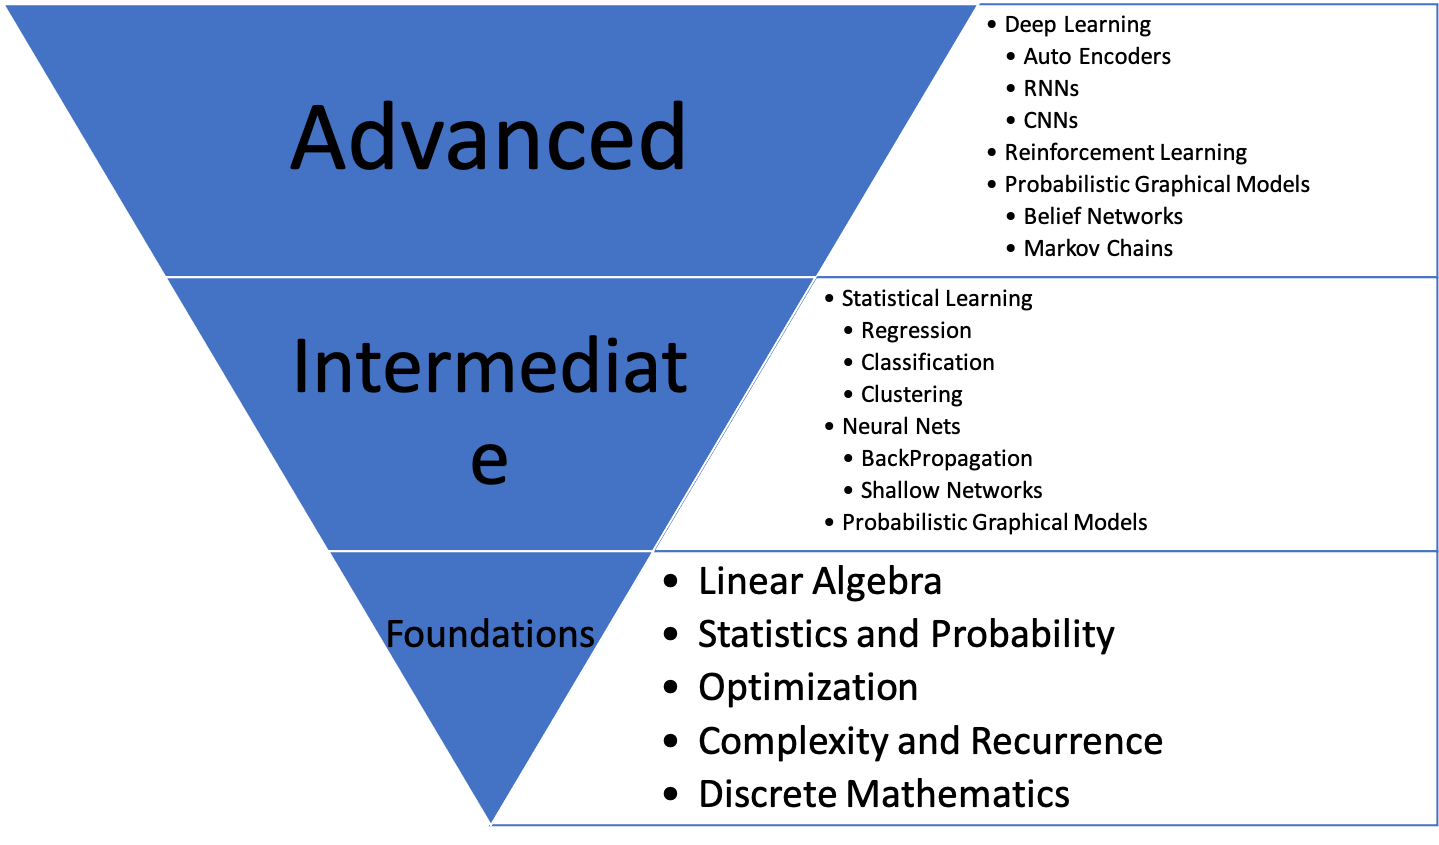
\includegraphics[scale=0.45]{AIPyramid.png}
\end{figure}
\framebreak
\end{frame}

\section{Getting started}
\label{sec:GettingStartedInML}
\begin{frame}[allowframebreaks]{Getting Started}
Artifical Intelligence
\begin{itemize}
\item \href{https://www.edx.org/course/cs50s-introduction-to-artificial-intelligence-with-python}{CS50's Introduction to Artificial Intelligence with Python (Harvard on edX)}
\item \href{http://aima.cs.berkeley.edu/}{Artificial Intelligence: A Modern Approach by Peter Norvig}
\end{itemize}
Machine Learning and Advanced ML
\begin{itemize}
\item \href{https://www.datacamp.com/tracks/machine-learning-fundamentals-with-python}{Machine Learning Fundamentals with Python (Datacamp)}
\item \href{https://www.edx.org/course/machine-learning-with-python-from-linear-models-to?index=product&queryID=3236d952a8cb57394e4415a111bcecb8&position=17}{Machine Learning with Python: from Linear Models to Deep Learning (MIT on edX)}
\item \href{https://www.edx.org/course/learning-from-data-introductory-machine-learning?index=product&queryID=19fa68b3b5207bdf2fb026fc68b342f9&position=1}{Learning From Data (CalTech on edX)}
\item \href{https://www.coursera.org/specializations/deep-learning}{Deep Learning Specialization (Deeplearning.ai)}
\item \href{https://www.coursera.org/specializations/probabilistic-graphical-models?}{Probabilistic Graphical Models Specialization (Coursera)}
\item \href{https://www.coursera.org/learn/introduction-tensorflow/}{Introduction to TensorFlow for AI, Machine Learning, and Deep Learning (Coursera)}
\end{itemize}
\framebreak
Foundations
\begin{itemize}
\item \href{https://math.mit.edu/~gs/linearalgebra/}{\textit{Introduction to Linear Algebra}} (Book) and \href{https://ocw.mit.edu/courses/mathematics/18-06sc-linear-algebra-fall-2011/}{\textit{Linear Algebra (18.06)} by Gilbert Strang (MIT)} (Online Course)
\item \href{https://www.pearson.com/us/higher-education/program/De-Groot-Probability-and-Statistics-4th-Edition/PGM146802.html}{\textit{Probability and Statistics} by Morris H. DeGroot, Mark J. Schervish} (Book)
\item \href{https://web.stanford.edu/~boyd/cvxbook/}{\textit{Convex Optimization}} (Book) and \href{https://online.stanford.edu/courses/soe-yeecvx101-convex-optimization}{\textit{Convex Optimization} by Stephen Boyd (Stanford)} (Online Course)
\item \href{https://www.edx.org/course/introduction-to-probability}{\textit{Introduction to Probability} (on edX) by Joseph Blitzstein (Harvard)} (Online Course)
\item \href{https://www.edx.org/course/probability-and-statistics-in-data-science-using-p?index=product&queryID=02cb349c3a3c75485697e8018465f1e4&position=2}{\textit{Probability and Statistics in Data Science using Python} (on edX) by Alon Orlitsky and Yoav Freund (UC San Diego)} (Online Course)
\end{itemize}
\end{frame}

% \section{Thanks}
\begin{frame}
\begin{center}
\Huge \(\textit{Thank You}\)\\
\Large \(\textit{Questions?}\)\\
\newline\newline\newline
\begin{table}[]
\begin{tabular}{l l}
{
\includegraphics[width=2.5ex]{LinkedIn-InBug-2C.png}}  \href{https://www.linkedin.com/in/vmeru}{\texttt{ linkedin.com/in/vmeru}}\\
\raisebox{-0.40ex}{
\includegraphics[width=2.5ex]{Octocat.png}}  \href{https://github.com/vrdmr}{\texttt{ github.com/vrdmr}} \\
\raisebox{-0.40ex}{
\includegraphics[width=2.5ex]{Twitter_logo_blue.png}}  \href{https://twitter.com/vrdmr}{\texttt{ @vrdmr}} \\
\end{tabular}
\end{table}
\end{center}
\end{frame}

% \section{References}
% \begin{frame}{References}
% \end{frame}
\end{document}